\documentclass[tikz,border=8pt]{standalone}
\usepackage{tikz}
\usetikzlibrary{positioning,arrows.meta,fit,backgrounds}

\begin{document}
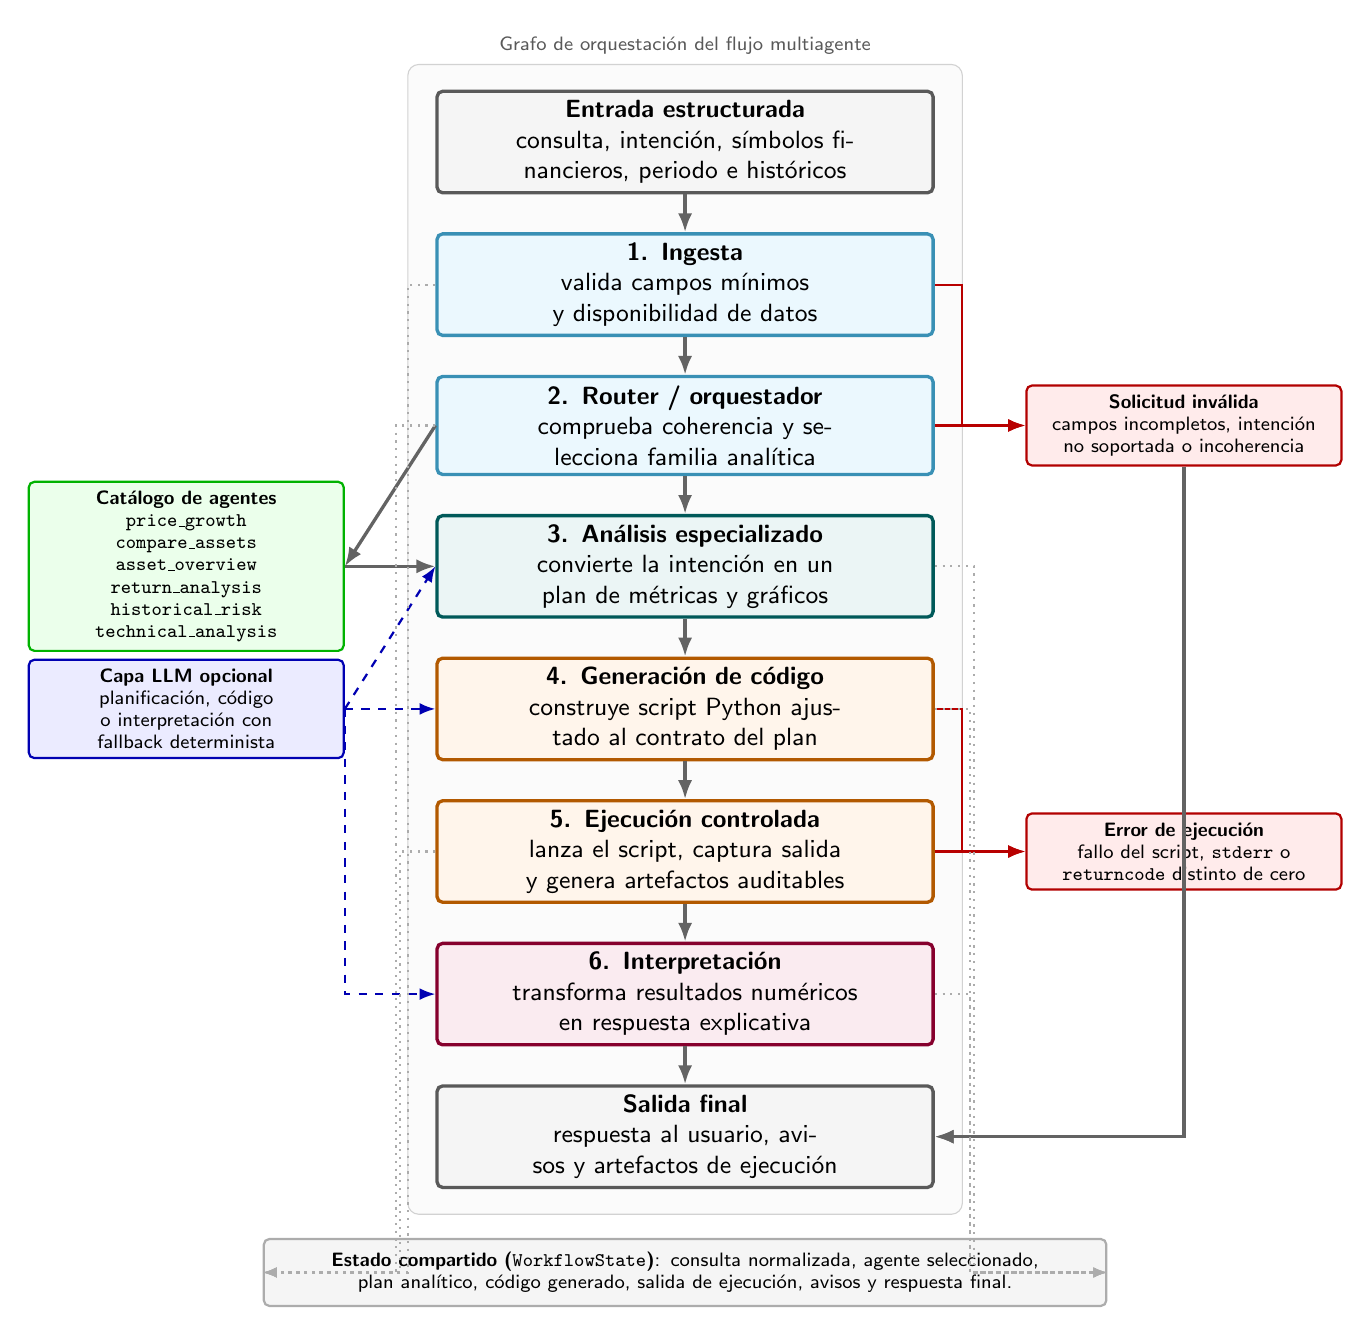
\begin{tikzpicture}[
    font=\sffamily\small,
    node distance=0.48cm,
    main/.style={
        draw=#1!70!black,
        fill=#1!8,
        rounded corners=2pt,
        very thick,
        align=center,
        minimum width=6.3cm,
        minimum height=0.92cm,
        text width=5.8cm
    },
    side/.style={
        draw=#1!70!black,
        fill=#1!8,
        rounded corners=2pt,
        thick,
        align=center,
        minimum width=4.0cm,
        minimum height=0.82cm,
        text width=3.65cm,
        font=\sffamily\scriptsize
    },
    statebox/.style={
        draw=gray!65,
        fill=gray!8,
        rounded corners=2pt,
        thick,
        align=center,
        minimum width=10.7cm,
        minimum height=0.85cm,
        text width=10.2cm,
        font=\sffamily\scriptsize
    },
    arrow/.style={-{Latex[length=2.4mm]}, very thick, draw=gray!78!black},
    errorarrow/.style={-{Latex[length=2.2mm]}, thick, draw=red!72!black},
    optionarrow/.style={-{Latex[length=2.0mm]}, dashed, thick, draw=blue!70!black},
    statearrow/.style={-{Latex[length=1.8mm]}, dotted, thick, draw=gray!65}
]

\node[main=gray] (input) {\textbf{Entrada estructurada}\\consulta, intenci\'on, s\'imbolos financieros, periodo e hist\'oricos};
\node[main=cyan, below=of input] (ingest) {\textbf{1. Ingesta}\\valida campos m\'inimos y disponibilidad de datos};
\node[main=cyan, below=of ingest] (router) {\textbf{2. Router / orquestador}\\comprueba coherencia y selecciona familia anal\'itica};
\node[main=teal, below=of router] (specialist) {\textbf{3. An\'alisis especializado}\\convierte la intenci\'on en un plan de m\'etricas y gr\'aficos};
\node[main=orange, below=of specialist] (codegen) {\textbf{4. Generaci\'on de c\'odigo}\\construye script Python ajustado al contrato del plan};
\node[main=orange, below=of codegen] (execution) {\textbf{5. Ejecuci\'on controlada}\\lanza el script, captura salida y genera artefactos auditables};
\node[main=purple, below=of execution] (interpretation) {\textbf{6. Interpretaci\'on}\\transforma resultados num\'ericos en respuesta explicativa};
\node[main=gray, below=of interpretation] (output) {\textbf{Salida final}\\respuesta al usuario, avisos y artefactos de ejecuci\'on};

\node[side=red, right=1.15cm of router] (invalid) {\textbf{Solicitud inv\'alida}\\campos incompletos, intenci\'on no soportada o incoherencia};
\node[side=red, right=1.15cm of execution] (execerror) {\textbf{Error de ejecuci\'on}\\fallo del script, \texttt{stderr} o \texttt{returncode} distinto de cero};

\node[side=green, left=1.15cm of specialist] (agents) {\textbf{Cat\'alogo de agentes}\\\texttt{price\_growth}\\\texttt{compare\_assets}\\\texttt{asset\_overview}\\\texttt{return\_analysis}\\\texttt{historical\_risk}\\\texttt{technical\_analysis}};
\node[side=blue, left=1.15cm of codegen] (llm) {\textbf{Capa LLM opcional}\\planificaci\'on, c\'odigo o interpretaci\'on con fallback determinista};

\node[statebox, below=0.62cm of output] (state) {\textbf{Estado compartido (\texttt{WorkflowState})}: consulta normalizada, agente seleccionado, plan anal\'itico, c\'odigo generado, salida de ejecuci\'on, avisos y respuesta final.};

\draw[arrow] (input) -- (ingest);
\draw[arrow] (ingest) -- (router);
\draw[arrow] (router) -- (specialist);
\draw[arrow] (specialist) -- (codegen);
\draw[arrow] (codegen) -- (execution);
\draw[arrow] (execution) -- (interpretation);
\draw[arrow] (interpretation) -- (output);

\draw[errorarrow] (ingest.east) -- ++(0.35,0) |- (invalid.west);
\draw[errorarrow] (router.east) -- (invalid.west);
\draw[errorarrow] (codegen.east) -- ++(0.35,0) |- (execerror.west);
\draw[errorarrow] (execution.east) -- (execerror.west);
\draw[arrow] (invalid.south) |- (output.east);
\draw[arrow] (execerror.south) |- (output.east);

\draw[arrow] (router.west) -- (agents.east);
\draw[arrow] (agents.east) -- (specialist.west);

\draw[optionarrow] (llm.east) -- (specialist.west);
\draw[optionarrow] (llm.east) -- (codegen.west);
\draw[optionarrow] (llm.east) |- (interpretation.west);

\draw[statearrow] (ingest.west) -- ++(-0.35,0) |- (state.west);
\draw[statearrow] (router.west) -- ++(-0.50,0) |- (state.west);
\draw[statearrow] (specialist.east) -- ++(0.50,0) |- (state.east);
\draw[statearrow] (codegen.east) -- ++(0.45,0) |- (state.east);
\draw[statearrow] (execution.west) -- ++(-0.45,0) |- (state.west);
\draw[statearrow] (interpretation.east) -- ++(0.45,0) |- (state.east);

\begin{scope}[on background layer]
\node[
    draw=gray!35,
    fill=gray!3,
    rounded corners=4pt,
    inner xsep=0.35cm,
    inner ysep=0.32cm,
    fit=(input)(ingest)(router)(specialist)(codegen)(execution)(interpretation)(output),
    label={[font=\sffamily\scriptsize, gray!70!black]above:Grafo de orquestaci\'on del flujo multiagente}
] {};
\end{scope}

\end{tikzpicture}
\end{document}
